\documentclass[11pt,a4paper]{article}
\usepackage[margin=1in]{geometry}
\usepackage{amsmath,amssymb,booktabs,array,graphicx,xurl,hyperref}
\usepackage[table]{xcolor}
\usepackage{natbib}
\usepackage[section]{placeins}
\usepackage{enumitem}
\usepackage[font=small,labelfont=bf,labelsep=period,justification=raggedright,singlelinecheck=false]{caption}
\hypersetup{colorlinks=true,linkcolor=blue,citecolor=blue,urlcolor=blue,
pdftitle={Online Appendix to Circular Capital in the Artificial Intelligence Stack},
pdfauthor={Anonymous}}
\setcitestyle{authoryear,round}
\setlength{\bibhang}{0.5in}
\graphicspath{{../figures/}}
\setlength{\parskip}{0.5em}
\rowcolors{2}{gray!10}{white}
\title{Online Appendix to\\ Circular Capital in the Artificial Intelligence Stack:\\ A Game-Theoretic Analysis of Market Power, Financial Fragility, and Welfare}
\author{Anonymous for double-blind review}
\date{}
\begin{document}
\maketitle
\noindent\textit{This Online Appendix accompanies the main manuscript submitted to the 7th Financial Economics Meeting (FEM-2026) and, on the fast track, to the International Journal of Finance \& Economics. It contains the evidence-grading apparatus (Appendix~A), the retirement-exposure appendix (Appendix~B), and the assumptions, caveats, and BCR-arithmetic appendix (Appendix~C).}

\appendix
% Appendices carry the grading apparatus, assumptions, and caveats so the
% body advances predictions and positions without interruption.
\section{Confidence, Evidence Grades, and Likelihood Scale}\label{sec:appendix-confidence}
The registry in the main text tags every claim with a likelihood and an evidence grade. This appendix defines both scales and documents what backs each tag.

\emph{How seriously to take each claim.} Every numbered prediction carries two separate tags. \textbf{Likelihood} is the author's assessed
probability that the claim proves right, on the fixed scale in
Table~\ref{tab:likelihood-scale-appendix} --- a judgment in the forecasting tradition
(IPCC, Tetlock), not a model estimate. \textbf{Confidence} rates the quality
of the evidence behind that judgment (High = contracts plus surviving stress
tests; Medium = scenario arithmetic that moves with inputs; Low = no
evidentiary basis). Model vote-shares (16/16, 100\%, 65\%) measure
\emph{robustness}, and formation scores (82.9\% etc.)\ measure
\emph{vulnerability} --- neither is the probability of the event. The two
numbers that look most like probabilities in this paper are therefore the
two you must not mistake for forecasts; the actual event probabilities are
the author's, stated in the registry.

\begin{table}[htbp]
\centering
\caption{Likelihood scale for author-assessed probabilities. Used only in the prediction registry of the main text; nowhere else in the paper does a percent sign denote an event probability.}
\label{tab:likelihood-scale-appendix}
\begin{tabular}{lc}
\toprule
Wording & Assessed probability \\
\midrule
Very likely & 85--95\% \\
Likely & 65--80\% \\
More likely than not & 50--65\% \\
Toss-up & $\sim$50\% \\
Unlikely & below 35\% \\
\bottomrule
\end{tabular}
\end{table}

\subsection{Evidence behind each likelihood}\label{sec:confidence}
A likelihood without a stated evidence grade is advertising. Table
below documents what each registry tag in the main text
rests on.

\emph{High confidence} requires a mechanism plus survival: the claim follows
from signed contracts (not sentiment or multiples) \emph{and} survives every
stress battery in the main text. Only P2 clears both bars ---
the ranking follows the contract book and holds 16/16 one-at-a-time with
100\% joint-draw agreement, so its $\sim$90\% is the paper's firmest number.

\emph{Medium confidence} means scenario arithmetic with stated parameters:
the direction is pinned down but the level moves with inputs. P1
($\sim$65\%) rests on three simultaneously present preconditions plus live
credit repricing (215bp, BBB-) --- strong pattern evidence, no base rate,
hence Likely rather than Very likely. P3 ($\sim$55\%) inherits two layers of
parameter uncertainty (impairment share, capex-cut share), so its honest
expression is the \$100--150B band, not the \$139.1B point. P5
($\sim$60\%) is capped by the formation rank's own weaker record (65\%
joint agreement, disclosed throughout). P6 ($\sim$60\%) assumes equity
buffers stay large; homogeneous GPU collateral is exactly the channel that
would break it. P7 ($\sim$70\%) rates the remedy \emph{order}, which survives
both the DWL and burst denominations --- the levels do not deserve the same
grade.

\emph{Low confidence} means no evidentiary basis exists. P8 is the only
resident: no timing model exists, so no probability is assigned.

\begin{table}[htbp]
\centering
\caption{Evidence behind each registry likelihood. Vote-shares are robustness checks, not event probabilities.}
    \label{tab:17-evidence-behind-each-registry}
\begin{tabular}{l>{\raggedright\arraybackslash}p{5.0cm}>{\raggedright\arraybackslash}p{5.2cm}}
\toprule
ID & Likelihood rests on & What would cut it in half \\
\midrule
P1 ($\sim$65\%) & 3/3 historical preconditions present; credit charging (215bp, BBB-) & Preconditions unwind without repricing \\
P2 ($\sim$90\%) & Contract incidence; 16/16 OAT; 100\% joint; seed + noise screens & Ranking flips on re-estimated exposures \\
P3 ($\sim$55\%) & Two-channel arithmetic on BEA GDP; capex share 86\% & Capex-cut share proves overstated \\
P4 ($\sim$70\%) & Densest round-trippers score highest (82.9\%) & First break lands elsewhere \\
P5 ($\sim$60\%) & Logit drivers; circular exposure dominates (w=1.6) & Joint agreement below 50\% on refresh \\
P6 ($\sim$60\%) & DebtRank x1.032 on large equity buffers & Fire-sale channel activates \\
P7 ($\sim$70\%) & BCR order stable across two denominations & Rank reversal in either table \\
P8 (none) & No timing model exists & --- \\
\bottomrule
\end{tabular}
\end{table}


\section{Who Holds the Wealth Channel: Retirement Exposure}\label{sec:appendix-retirement}
The \$19.1B wealth channel is computed at a uniform 4 cents of consumption
per dollar of equity loss. Two sourced facts qualify who bears it.
\emph{First, the exposure stock:} 401(k) equity funds hold \$3.7T and IRA
equity funds \$4.8T \citep{ici2026}; at the Magnificent-7's $\sim$34\%
S\&P~500 weight \citep{datatrek2025}, fund-held retirement equity carries a
$\sim$\$2.9T Big Tech slice --- a floor under a market-weight assumption
(hybrids, direct pension holdings, and taxable accounts excluded).
\emph{Second, the loss lands where the MPC is lowest:} the top decile holds
$\sim$87\% of equities \citep{feddfa2025}, while the Fed's heterogeneous
estimates put top-quintile MPC at 0.8 cents against 7.5 cents for the bottom
80\% \citep{fedfeds2025}.

Rerunning the paper's own \$477.5B implied market-cap loss (\$19.1B / 0.04)
through holder-weighted MPCs gives a \$6.1--7.0B consumption memo
(Fig.~\ref{fig:retirement-exposure}, right panel; full arithmetic in
\texttt{tables/backtest/retirement\_exposure.csv}, built by
\texttt{build\_retirement\_exposure.py} from live Table~7.12 values). The
reading cuts against alarmism on the aggregate: the uniform 4-cent
assumption \emph{overstates} the consumption drag, because wealthy holders
absorb most of the loss at 0.8 cents. The GDP headline stands at \$139.1B;
the memo combined figure is $\sim$\$126--127B.

The contraction risk is compositional, not larger. The \$33--48B
balance-sheet slice landing on 7.5-cent households is a
retirement-adequacy shock, and a consumption flow understates the welfare
loss for near-retirees drawing fixed balances. Three fringe channels widen
that slice beyond fund-held equity: US private credit ($\sim$\$1.7--1.8T)
with listed BDCs ($\sim$\$500B) near \$0.78 per \$1.00 of NAV and retail
private-credit assets up 43.7\% since end-2024 \citep{pitchbook2026}; public
pensions pushing into private markets (CalPERS: private equity 17\%,
private debt 8\%) \citep{calpers2025}; and GPU-collateralized neocloud debt
(CoreWeave \$14--19B, interest near a third of revenue) \citep{techcrunch2026}
--- the collateral class the top-BCR remedy caps. Executive Order 14330
(August~2025) opening 401(k)s to alternatives accelerates all three
\citep{eo14330}.

\begin{figure}[htbp]
\centering
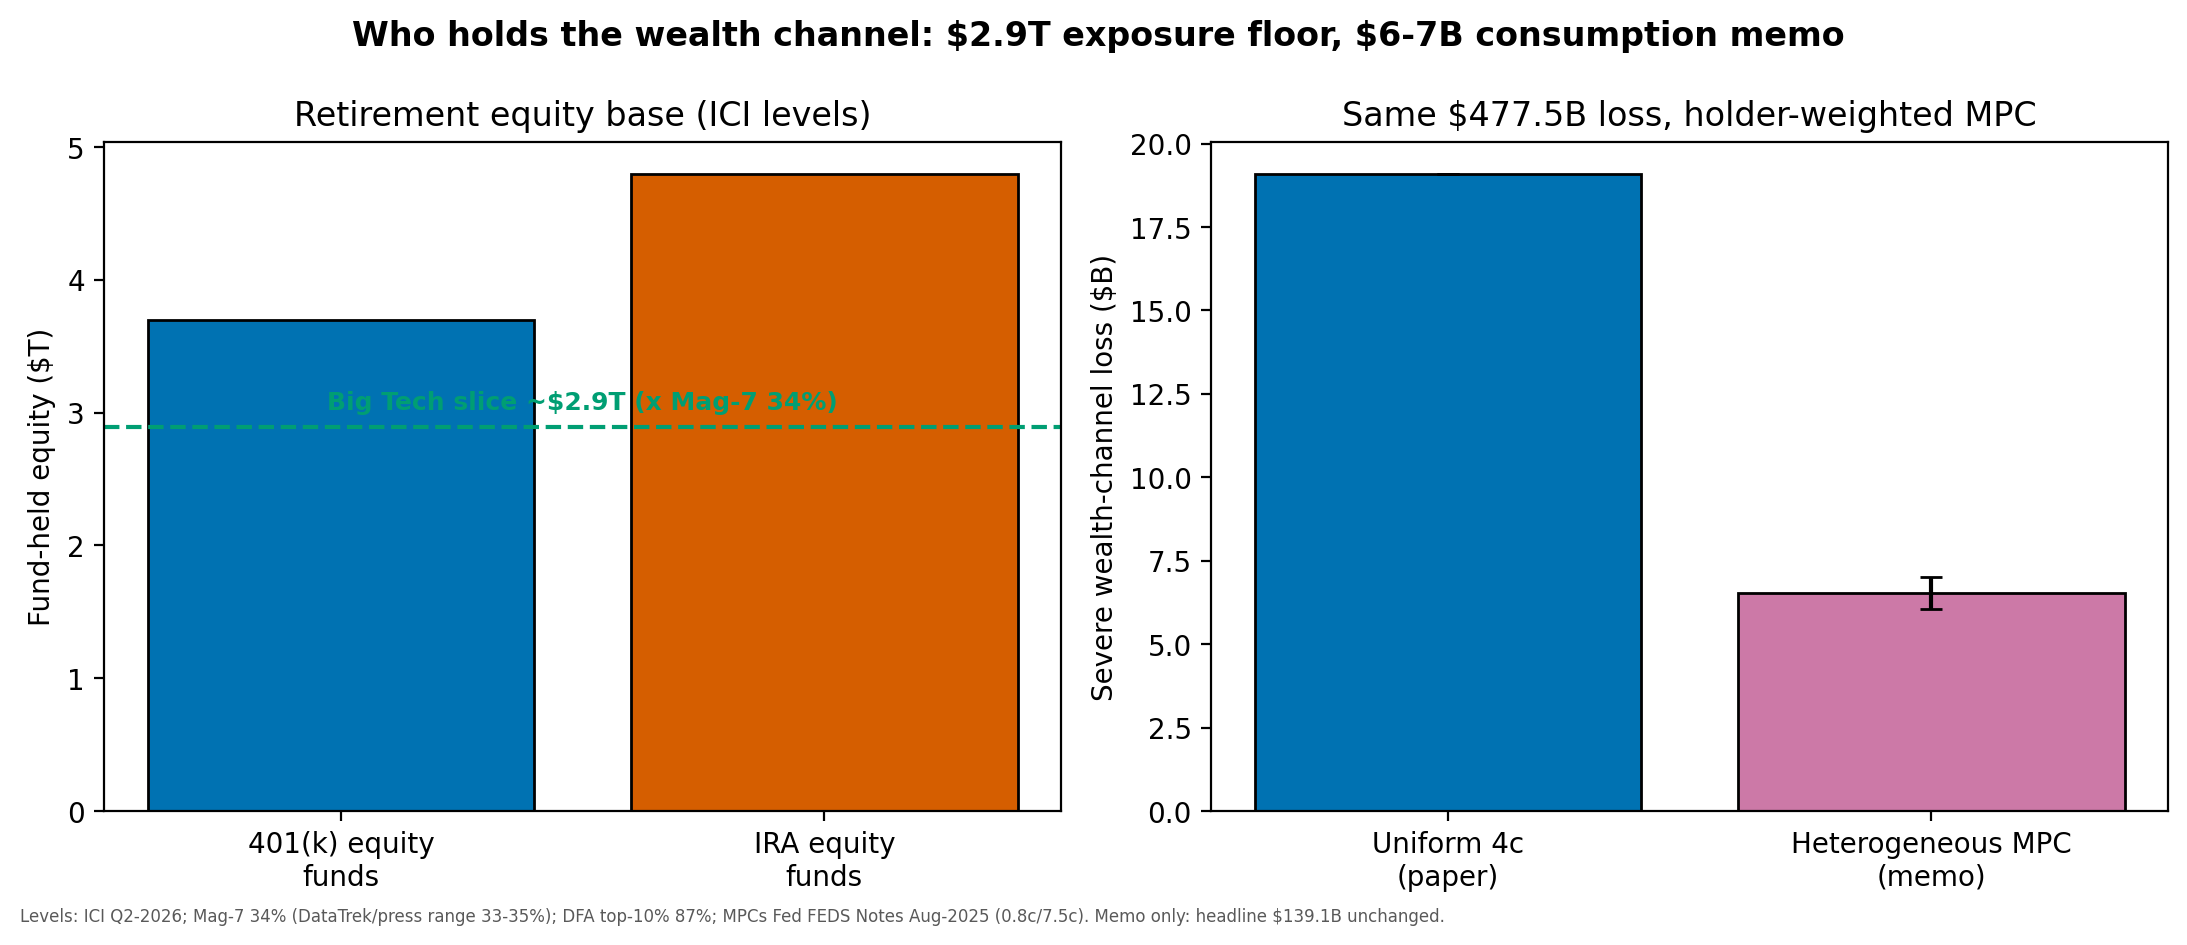
\includegraphics[width=0.9\textwidth,height=0.82\textheight,keepaspectratio]{retirement_exposure.png}
\caption{Left: the retirement equity base behind the wealth channel (ICI Q2-2026 levels); the dashed line is the $\sim$\$2.9T Big Tech slice at a 34\% index weight --- a floor. Right: the same \$477.5B equity loss under the paper's uniform 4-cent MPC versus holder-weighted MPCs (0.8c top quintile, 7.5c rest) --- the aggregate drag shrinks while its incidence concentrates on retirement holders.}
    \label{fig:retirement-exposure}
\end{figure}

\section{Assumptions, Caveats, and Updating Protocol}\label{sec:appendix-assumptions}\label{sec:limits}
The games are static and one-shot, missing learning and entry; the cascade
is static reverberation, not dynamic clearing; the GDP math is
US-calibrated without multipliers; formation odds are scenario scores, not
measured probabilities.
Policy BCRs are ex-ante engineering estimates with scenario-assumed
reduction rates, not revealed-preference measures; their ordering is more
credible than their levels, and prevention is priced, not distributional
incidence. Chinese open-weight systems are excluded by the China-labs rule:
the published formation odds carry no open-source margin-compression
channel, which instead runs as an explicit scenario, while Chinese labs
themselves contribute no edge to the frame. Geography porting exists as
stated scenarios (Table~7.19) still awaiting local vintages. Treat every
dollar figure as a marker and every ranking as the claim. When
funding rounds reprice, tranches activate, or spreads gap, re-run the
pipeline: if the burst order moves, this prediction moves with it --- that
updatability is the difference between a standing warning and a stale one.


\subsection{BCR arithmetic, break-even conditions, and what the ratios omit}\label{sec:policy-bcr}
Every benefit--cost ratio in this paper is gross benefit over cost, computed
identically in both policy families and audited row by row in pipeline
Table~6.4. Welfare family: $B_s = \mathrm{DWL}\times r_s$, $N_s =
B_s - C_s$, $\mathrm{BCR}_s = B_s / C_s$ with $\mathrm{DWL} =
416.77\text{ billion USD}$; burst family: the same form with the severe burst total
(\$478.3B) as the denominator --- the two families must never be compared
rate-to-rate. The break-even reduction $r^* = C_\mathrm{base} /
\mathrm{denominator}$ is the effectiveness level at which the base-case
cost exactly pays for itself: welfare break-evens run 0.48\% (antitrust,
base 25\%), 0.72\% (data sharing, base 18\%), 1.20\% (interoperability,
base 35\%), 1.92\% (subsidies, base 22.5\%) and 3.60\% (combined, base
55\%); burst break-evens run 0.21\% (lending caps, base 12\%), 0.42\%
(disclosure, base 15\%), 1.25\% (reserve, base 10\%) and 1.88\%
(combined, base 30\%). Every base case clears its break-even by an order of
magnitude or more, and every welfare conservative case still pays
(BCR$\ge$1, lowest 5.2 for subsidies) --- so the \emph{ranking} survives
broad sensitivity even where the point levels should not travel. What the
ratios omit is stated, not hidden: costs and benefits are single-year and
undiscounted (no horizon or discount rate is estimated); incidence across
taxpayers, workers and users is outside the frame; implementation delay and
evasion are unmodeled; private-sector compliance costs, administrative
burdens and dynamic investment-incentive effects sit on the cost side only as
the narrow agency budgets in Table~6.4, so every BCR is gross of the
regulatory burden it would impose --- again favoring the ranking over the
level. Burst-family reduction rates are scenario
assumptions with mechanism analogies, not literature estimates.

\emph{Regulatory lift.} Disclosure should follow this paper's booking rule
--- committed face values reported, conditional tranches disclosed by
trigger --- which regulators can lift verbatim into reporting templates.
Competition screening should precede price policing (within-layer HHIs
4,057--5,632, all highly concentrated; cross-stack top-two share 86.2\%):
review consolidation and exclusivity clauses in the booked deal graph before
benchmarking cloud margins. The European Union offers the natural experiment
for the interoperability remedy: DMA enforcement data on portability
mandates can calibrate the reduction rates behind the 29.2 BCR, replacing
engineering assumptions with revealed compliance effects. Finally, keep the
ex-post shelf stocked --- public-cloud conversion designs, worker
protections, structural-reform statutes --- keyed to the severe-burst
trigger (\$139.1B GDP cost) this paper quantifies.

\renewcommand{\refname}{}
\section*{References}
All citations below follow APA style (6th edition) as required by the journal. Every entry is cited in this appendix; every in-text citation resolves below.

\begin{thebibliography}{99}

\bibitem[Board of Governors(2025)]{fedfeds2025}
Board of Governors of the Federal Reserve System. (2025).
Wealth heterogeneity and consumer spending.
\emph{FEDS Notes}, August~5, 2025 (top-quintile MPC 0.8 cents, bottom-80\%
7.5 cents per dollar of wealth).
Available at \url{https://www.federalreserve.gov/econres/notes/feds-notes/wealth-heterogeneity-and-consumer-spending-20250805.html}.

\bibitem[CalPERS(2025)]{calpers2025}
California Public Employees' Retirement System. (2025).
Private-markets allocation targets: private equity 17\%, private debt 8\%,
within a 40\% private-markets portfolio.
Board materials and press reporting, 2024--2025.

\bibitem[DataTrek via MarketWatch(2025)]{datatrek2025}
DataTrek Research via MarketWatch. (2025).
Magnificent Seven at 34\% of the S\&P~500 (December~2025 prints; 33--35\%
range through August~2026 press).
Reported October~21, 2025.

\bibitem[Federal Reserve DFA(2025)]{feddfa2025}
Board of Governors of the Federal Reserve System. (2025).
Distributional Financial Accounts: top decile (income-ranked) holds
$\sim$87\% of corporate equities and mutual fund shares (Q2 analysis).

\bibitem[Investment Company Institute(2026)]{ici2026}
Investment Company Institute. (2026).
Quarterly retirement market data, Q2~2026: total retirement assets
\$51.2T; 401(k) equity funds \$3.7T; IRA equity funds \$4.8T; government
defined-benefit assets \$10.4T; target-date fund assets \$4.86T (end-2025).

\bibitem[PitchBook / Morningstar(2026)]{pitchbook2026}
PitchBook; Morningstar. (2026).
Private-credit monitor: retail private-credit assets up 43.7\% since
end-2024; listed BDCs near \$0.78 per \$1.00 of NAV (2026 prints).

\bibitem[TechCrunch / PitchBook(2026)]{techcrunch2026}
TechCrunch; PitchBook. (2026).
CoreWeave debt obligations \$14--19B (Q3--September~2025 prints),
GPU-collateralized; quarterly interest near one-third of revenue.
Reported January~26, 2026.

\bibitem[White House(2025)]{eo14330}
White House. (2025).
Executive Order 14330, ``Democratizing Access to Alternative Assets for
401(k) Investors'' (August~7, 2025): directing DOL review of 401(k)
access to private equity, private credit, real estate, and digital assets.
\end{thebibliography}
\end{document}
